\section{Auswertung}
Für die Auswertung der Messdaten werden einige Fehlerrechnungen benötigt. Diese sind im Folgenden angegeben.
Alle Mittelwerte werden durch
\begin{equation}
\bar{x} = \frac{1}{N} \sum_{i=1}^{N} x_{i}
\end{equation}
bestimmt, wobei $N$ die Anzahl der betrachten Messwerte angibt. Die Standardabweichung $\sigma$ einer Messreihe lässt sich folgendermaßen berechnen.
\begin{equation}
\sigma = \sqrt{\frac{1}{N-1}\sum_{i=1}^{N} (x_{i} -\bar{x})^2 }
\end{equation}
Der sogenannte Standardfehler des Mittelwerts ist durch eine Beziehung zur Standardabweichung definiert.
\begin{equation}
\increment \bar{x} = \frac{\sigma}{\sqrt{N}} = \frac{1}{\sqrt{N}} \sqrt{\frac{1}{N-1}\sum_{i=1}^{N} (x_{i} -\bar{x})^2 }
\end{equation}
Wenn Werte in einer beliebigen Berechnungsformel fehlerbehaftet sind kann der Fehler anhand der Gaußschen Fehlerfortpflanzung ermittelt werden. Diese sieht im allgemeinen Fall folgendermaßen aus.
\begin{equation}
\increment f = \sqrt{\sum_{i=1}^{N} \left( \frac{\partial f}{\partial x_{i}}\right)^2 (\increment x_{i})^2}
\end{equation}
Es wird also über alle Variablen summiert welche einen Fehler $\increment x_{i}$ besitzen. Für Formeln mit nur einem fehlerbehafteten Wert vereinfacht sich die Gleichung dementsprechend.

\subsection{Statische Methode}


\begin{figure}
    \centering
    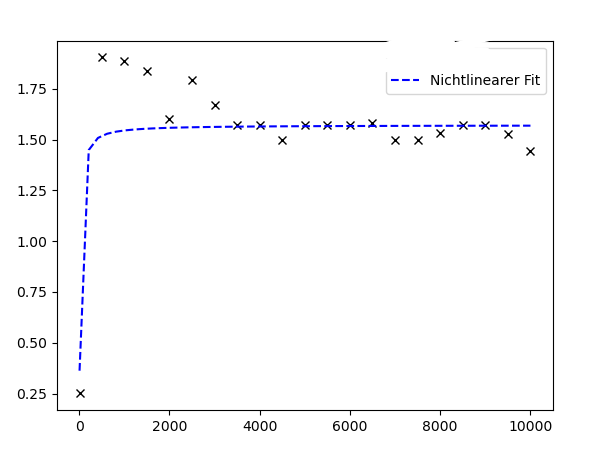
\includegraphics[width=\textwidth]{build/plot1.pdf}
    \caption{Temperaturverlauf der Messsonden T1 und T4 angebracht auf Messing} 
    \label{fig:plot1}
\end{figure}

\begin{figure}
    \centering
    \includegraphics[width=\textwidth]{build/plot2.pdf}
    \caption{Temperaturverlauf der Messsonden T5 (Aluminium) und T8(Edelstahl)} 
    \label{fig:plot2}
\end{figure}
